\subsection{Was ist Cloud Computing?}

\begin{figure}[h]
    \centering
    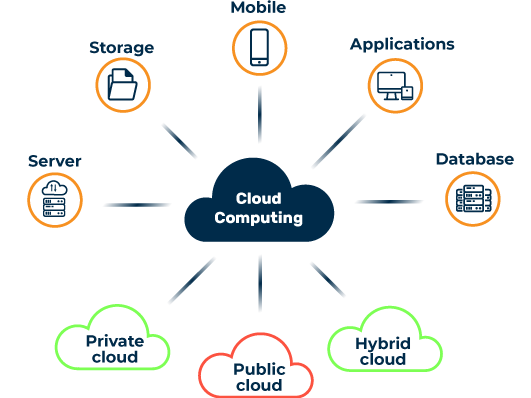
\includegraphics[scale=0.9]{sections/cloud-computing/images/cc.png}
    \caption{CC-Overview}
    \label{fig:kimldl-comparison}
\end{figure}

Cloud Computing ist ein Modell, bei dem virtueller Speicher, jegliche Art von Server, Anwendungen usw. nicht physisch, sondern rein über das Internet bereitgestellt werden. Diese werden in der Regel nach Bedarf als Teil eines As-a-Service-Modells angeboten. Üblicherweise wird dieses Modell in Verbindung mit nutzungsbasierter Bezahlung offeriert. Mithilfe der Cloud werden lokale Rechenzentren und interne Systeme mit virtuellen Rechen-, Netzwerk- und Speicherressourcen ausgetauscht. Im Normalfall werden diese Ressourcen von externen Anbietern bereitgestellt. Statt selbst breit gefächerte Rechen- und Speicherressourcen aufzustellen und nebenbei auch noch zu warten, wird eine Vielzahl dieser Aufgaben von einem Cloudservice-Anbieter übernommen.

\subsection{Vorteile von Cloud Computing}

Oft fallen, in Verbindung mit dem Thema Cloud Computing, Stichwörter wie „flexibel“ oder „agil“, das liegt daran, dass gerade in heutigen Zeiten marktseitige und auch technologische Veränderungen schnell und oft vorgenommen werden und deswegen Unternehmen oftmals nicht Schritt halten können. Deshalb betreiben viele Unternehmen sogenanntes Outsourcing, um nicht selbst für die Rechenleistung ihrer eigenen Dienste verantwortlich zu sein. Skalierbarkeit spielt hierbei eine große Rolle, zum Beispiel: je mehr Zugriffe auf einen Webshop, desto mehr Ressourcen müssen im Hintergrund hochgefahren werden, um eine fehlerfrei Nutzung zu garantieren.

Auch die Usability ist simpler bei cloudbasierten Prozessen, da viele dieser Prozesse in den Hintergrund verschoben und von den Cloud Service-Anbietern übernommen werden. Der Aufwand für Wartung, Beschaffung, usw. für Rechenzentren entfällt weitgehend. Somit kann man im Bereich Energie- und Erhaltungskosten einsparen. Im Allgemeinen werden die Kosten für solche Dienste je nach Vereinbarung nutzungsabhängig vereinbart. Im Normalfall fallen diese Kosten monatlich oder jährlich an, wobei diese verhältnismäßig kleiner als die von On-Premise Lösungen sind.

Ebenfalls ein wichtiges Stichwort hier ist Datenkonsistenz. Im Fall von komplexen Prozessen ist die Konsistenz der Daten ein wesentlicher Punkt, um drastische Probleme zu verhindern. Gerade bei dezentraler Speicherung und Verarbeitung der Daten, ist die Synchronität sehr wichtig. Bei Cloud Computing ist dieses Risiko minimiert, da im Normalfall die Daten, auch bei Zugriff von unterschiedlichen Schnittstellen, synchron sind.

\subsection{Hindernisse für den Einsatz einer Cloud}

Da es sich beim Cloud Computing um ein neues Modell handelt, besteht eine gewisse Unsicherheit, wie man auf allen Ebenen eine solide Sicherheit erreichen kann. Deshalb wird die Fähigkeit der Cloud, den Datenschutzbestimmungen gerecht zu werden, in Frage gestellt. Das Grundprinzip der Cloud sieht eine dauerhafte Verfügbarkeit vor und gerade diese Verfügbarkeit kann auch ein großer Nachteil sein. Erst durch den offenen Zugang zu den zur Verfügungen gestellten Rechenleistung und anderen Ressourcen, entfaltet das CC-Model sein volles Potenzial. 

Heutzutage müssen Anwendungen dauerhaft erreichbar sein und hierbei kann sich die Abhängigkeit von einem Cloud Service Provider negativ auf dauerhafte Konnektivität auswirken. Im Fall eines Ausfalls oder von Aussetzern müssen Notfallpläne- und oder Ressourcen gestartet werden um, zum Beispiel Datenverlust zu verhindern, was im Allgemeinen, zu fatalen Fehlern führen kann.

%https://www.ias.uni-stuttgart.de/service/begriffslexikon/bedeutung-der-interoperabilitaet-fuer-das-internet-der-dinge/
Die Interoperabilität und Übertragbarkeit von Informationen zwischen privaten und öffentlichen Clouds sind entscheidende Voraussetzungen für die breite Einführung von Cloud Computing in Unternehmen. Viele Unternehmen haben erhebliche Fortschritte bei der Standardisierung ihrer Prozesse, Daten und Systeme durch die Einführung von ERPs gemacht. Dieser Prozess wurde ermöglicht durch skalierbare Infrastrukturen, zur Schaffung einzelner Instanzen oder hochintegrierter Verbindungen zwischen Instanzen, um die Konsistenz von Stamm- und Bewegungsdaten zu verwalten und zuverlässige konsolidierte Informationen zu erzeugen.
